\chapter{Conceptualising Emergence}\label{Yangbenn}
\label{ch2}
In this chapter, we walk through multiple aspects of acquiring\is{acquisition} an adult phonology from the infant learner's perspective. We begin with the challenge of identifying the segments of the language being learned, then turn to its discrete vowel categories and how those categories\is{category} are cross-classified. The distribution of Yangben\il{Yangben|(} vowels raises issues of phonetic\is{phonetics} concreteness and the role of phonological patterns in establishing segment classes (addressed in \Sec\ref{Yangben_categories_section}), two issues that  play a central role in our discussion. Yangben ([\ipa{jàŋb\`{ɛ}n}]), also referred to as Kalong ([\ipa{kàl\ipa{\`{ɔ}}ŋ}]), is a member of the Mbam group\il{Mbam group} of Bantu\il{Bantu} languages spoken in Cameroon\is{Cameroon}, classified as Bantu A62 by \citet{Guthrie:1967-71},  glottocode yang1293. Our analysis builds on earlier investigations by \citet{Paulian:1986} and \citet{Hyman:2003kalong}, but depends primarily on \citet{Boyd:2015}.

There is something of a back story to our choice of Yangben for this basic demonstration of the {Emergent framework} -- fundamentally this demonstration could be made with any language. Our initial interest in Yangben stemmed from the work of \citet{Paulian:1986} and \citet{Hyman:2003kalong}. What was intriguing was their argument that the language would require the postulation of abstract vowels\is{vowels!abstractness} to determine phonological patterns of importance where the relevant vowels were not distinguished phonetically.\is{phonetics} As it turns out, however, \citet{Boyd:2015} demonstrates that the ``abstract''\is{abstractness} vowels of Yangben are actually phonetically motivated. Boyd's description and analysis differ importantly from the earlier literature in that she identifies high retracted vowels, [\ipa{ɪ, ʊ}], vowels whose existence had been expected for phonological reasons and which she documents both phonologically and phonetically. Hence Boyd  proposes a nine-vowel system\is{inventory!Yangben} in contrast to earlier analyses of Yangben with a seven-vowel system. For our purposes, this means that Yangben moves from being an example of required abstractness to relatively mundane concreteness.

In addition, vowel distribution\is{distribution!Yangben vowels} in Yangben illustrates issues involved in building words by compiling smaller parts,\is{word} or morphs\is{morph}, addressed in Chapter \ref{Yangben_assessment_section}.  Together, the discussion in these two chapters demonstrates both that it is possible to develop a grammar\is{Emergent Grammar} without significant recourse to universal innate principles, and that {such a grammar\is{grammar} can resolve complex challenges} to classical innateness-based phonological analysis.\is{innateness} 


Our initial focus is  identifying  the nine contrastive\is{contrast!vowels} vowels in Yangben and their relevant classification. We show here that some of the motivation for their classification is phonetic\is{phonetics} (\Sec\ref{Yangben_categories_section}), how this classification is represented in grammatical categories (\Sec\ref{section_natural_classes}), and, finally, that some of the motivation for such categories is phonological (\Sec\ref{intro-partitions-sec}).

\section{Acquiring discrete sound categories}\label{Yangben_categories_section}\is{category}\is{acquisition!sets}\is{set!acquisition}
We sketch here in an idealised fashion how hearing and remembering,\is{memory} identifying similarities\is{similarity} and generalising\is{generalisation!acquisition} over what is stored can lead to a phonological grammar of a vowel  system.\is{inventory!vowel}  For a language to be learnable\is{learnability} at all, the data must be sufficient for each learner to acquire\is{acquisition} knowledge of the particular segments and patterns encountered: what a learner hears must ultimately include sufficient information for phonological acquisition.\is{acquisition} We demonstrate here the viability of our claim, that an adequate, predictive adult phonological grammar\is{grammar} is possible to be acquired without appeal to innate linguistic principles.\is{innateness}\footnote{See \citet{Weijer:2017} for a similar demonstration, looking into the acquisition\is{acquisition} of a constraint against complex onsets in English.\il{English}}
 
 
The symbols in \tabref{Yangben-vowels} represent the vowel\is{vowels!Yangben} qualities of Yangben\is{symbol}  that the Yangben learner must acquire; these are the symbols  used in \citet{Boyd:2015}, representing the nine vowel qualities cross-cut by two lengths and two tones. 

\begin{table} 
\caption{Yangben vowels\label{Yangben-vowels}}
\begin{tabular}{lcccccc}
\lsptoprule
            &\multicolumn{2}{c}{front}	&central	&\multicolumn{2}{c}{back/round}\\\midrule
advanced	&\ipa{{\í}/{\í}ː/{\ì}/{\ì}ː}	&é/\ipa{éː}/è/\ipa{èː}	&	&ó/\ipa{óː}/ò/\ipa{òː}	&ú/\ipa{úː}/ù/\ipa{ùː}\\
retracted	& \'{ɪ}/\'{ɪ}ː/\`{ɪ}/\`{ɪ}ː	&\ipa{\'{ɛ}/\'{ɛ}ː}/\ipa{ \`{ɛ}/\`{ɛ}ː} 	&~ ~ á/\ipa{áː}/à/\ipa{àː} ~ ~	&\ipa{\'{ɔ}/\'{ɔ}ː}/\ipa{\`{ɔ}/\`{ɔ}ː} &\ipa{\'{ʊ}/\'{ʊ}ː}/\ipa{\`{ʊ}/\`{ʊ}ː}\\
\lspbottomrule
\end{tabular}
\end{table}

An early challenge for the language learner is to perceive and identify these 36 distinct vocalic categories, a necessary  stage in acquisition\is{acquisition} regardless of whether or not there are innate linguistic principles. For our discussion, we assume that the learner's pool of knowledge has grown to approach an amount sufficient to at least begin to identify acoustically distinct, sometimes contrastive,\is{contrast!vowels} vowels.

\begin{dadpbox}{Are language sound categories evidence of linguistic human cognition?}{box-sound-categories-innateness}
As has been known since the 1970s, there is agreement between humans and some other animals\is{nonhuman species} for at least some sound \is{category}categories.\is{cognition!animal} \citet{Kuhl+:1975} and \citet{Kuhl+:1982macaques} show that chinchillas and macaques categorise a /ba/-/pa/ continuum in the same way as very young infants (1 and 4 month-olds), \citet{Eimas+:1971}. \citet{Kluender+_1987} show Japanese quail\is{nonhuman species} have a sophisticated categorisation of [t] and [d] regardless of phonetic\is{phonetics} effects of following vowels. Acquiring\is{acquisition} sound categories of particular types may be part of human cognition,\is{cognition} but it is not exclusive to humans, and so is not necessarily evidence of human cognition specific to language. 
\end{dadpbox}

Our suppositions in this domain are reminiscent of both exemplar models\is{Exemplar Theory} (\citealt{Lacerda:1995, Lacerda:1998, Pierrehumbert:2001ed, Johnson:2007, Cole:2009}; see also \citealt{Weijer:2009, vandeWeijer:2012} on coupling Optimality Theory\is{Optimality Theory} and Exemplar Theory) and self-organising systems\is{self-organising system}  \citep{deBoer:2000selforg, Lin:2005, Wedel:2007}. We assume that a Yangben  learner\is{acquisition!early} hears and remembers parts of the ambient speech. To ``hear and remember''\is{memory} requires the learner to identify at least a chunk\is{chunk} of an utterance and mentally store that chunk. In the earliest learning, only small chunks\is{chunk} of language sound may be remembered. Some of these will correspond neatly to vowels,\is{vowels!acquisition} while other chunks may correspond to consonants, or to transitions,\is{transitions} chunks\is{chunk} that span both part of a vowel and part of a consonant. For example, a Yangben  learner hearing \ipa{[n\`{ɪ}pàná]} `{\sc c5}-foot' may perceive\is{perception} and retain (some of) the vowel chunks\is{chunk!vowels} [\`{ɪ}], [à], and [á], and (some of) the consonant chunks\is{chunk} [n] and [p].\footnote{Yangben,  as is typical of Bantu languages, exhibits noun classes; `{\sc c5}' refers to noun class 5.} But the learner may also retain chunks\is{chunk} that span C-V transitions,\is{transitions} getting units like [\ipa{n\`{ɪ}}], or [\ipa{\`{ɪ}p}], or [\ipa{pá}], or some subpart thereof.

There are numerous differences among the items that are acquired:\is{acquisition!early} each token is physically distinct from all other tokens (uttered at different times, by different people, at different volumes, etc., as well as the possibility of being phonologically different). At the same time, there are some tokens bearing similarities.\is{similarity!acquistion} As shown in \citet{Lindblom:2000}, incidences of physical properties cluster in some areas and are sparse in others, urging identification of certain similarities due to density in the observational space. Thus, as more items are acquired, the frequency of chunks\is{chunk!frequency} corresponding most closely to single vowels are highly likely to exceed the frequency\is{frequency} of certain other types of chunks,\is{chunk} due to the nature of the input. As a point of reference, consider the F1/F2 chart in \figref{Yangben-formants}, from \citet{Boyd:2015}. The vowels represented here also vary along dimensions  that are not shown in this figure -- whether the vowel is long or short, and whether the vowel is high-toned or low-toned. The challenge for the learner is to sort out this multidimensional space.\is{acquisition!sounds} We simplify the discussion here by focussing only on F1 and F2, only two of the multiple relevant dimensions, the two shown in \figref{Yangben-formants}.\is{acoustics!Yangben}\is{acoustics!vowels}

\begin{figure} 
\caption{Acoustics of Yangben vowels, from \citet[238]{Boyd:2015}\label{Yangben-formants}}
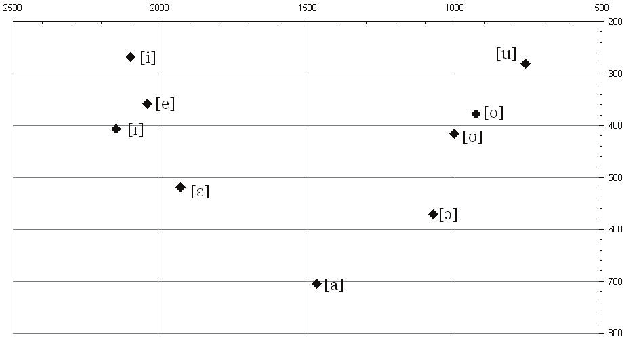
\includegraphics[width=\textwidth]{images/Yangben_acoustics_Boyd_2015.pdf}
\end{figure}

Each vowel\is{vowels} ``point'' on the chart in \figref{Yangben-formants} corresponds to a cloud of observations, with large gaps\is{gap} where tokens are non-existent or rare. \citet{Lacerda:2003} shows that the search space is enormous, so that clusters of similar\is{similarity!acquisition} sounds really stand out.  \citet{Gerken+:2015} demonstrates that learning can be accomplished based even on a single surprising input. Putting these two together, here the surprise is finding more than one token in a particular area of the search space. The stage is set for  the human drive to find and generalise\is{generalisation!category} over similarities: the learner creates categories of similar items based on  acoustic properties,\is{acquisition!sounds} resulting in vowel categories.\is{category}\footnote{There are fewer vowel qualities than consonant types in most if not all languages  (\citealt{Ladefoged+:1996}) and syllables typically have at least one vowel, so tokens of individual vowels\is{vowels} occur with higher frequency\is{frequency}\is{acquisition!frequency} than do tokens of individual consonants, correctly predicting that learners will generally hone in on vowels first (\citealt{Kuhl+:1992, Polka+:1994}).} To summarise, by remembering and storing\is{memory}, learners acquire\is{acquisition!sets}\is{set!acquisition} dense clusters of chunks,\is{chunk} primitive vowel categories.\is{category} Recognising that the chunks\is{chunk} in each cluster are similar\is{similarity!acquisition} to each other and generalising\is{generalisation!acquisition} over that similarity leads to the initial abstract\is{abstractness} representation of each vowel\is{vowels!categories} category.\footnote{We assume that learning  consonants is similar to learning  vowels as discussed here, with the added complexity of determining place from transitions\is{transitions} to adjacent vowels. As with vowels,  snippets of consonant sounds which include pieces of multiple consonants will have low frequency and so will lack reinforcement as a relevant unit.}

\begin{dadpbox}{Generalising and attention to detail}{box-detail-&-generalisation}
Assuming a role for some version of Exemplar Theory\is{Exemplar Theory}, we hypothesise that a great deal of phonetic\is{phonetics} detail is recorded in the relevant memory\is{memory!exemplar cloud} traces that make up each cloud.  Categorisation\is{category} over multiple distinct tokens focusses on shared similarities; by grouping units sharing properties, the fine detail defining particular exemplars comes to hold less importance. Similarities\is{similarity!acquisition} may define cross-cutting categories\is{category} for a single set of forms. For example, [\ipa{{\ì}, {\ì}ː, {\í}, {\í}ː}] might form an ``i'' category, while [\ipa{{\ì}, {\í}, \`{ɪ}, \'{ɪ}, è, é, ...}] might form the category of short vowels, and so on. Categories could be established by sharing advanced or retracted tongue root, high or low tone, particular F1 values, etc. Categorisation, however, does not mean loss of observed detail; rather, categorisation simply provides a means of grouping individual units based on shared properties.\is{generalisation}\is{attention}
\end{dadpbox}

To ground this with Yangben  data, suppose the learner acquires\is{acquisition!frequency} the forms in  (\ref{Yangben-random-vowels}). This set contains all nine vowel qualities found in Yangben,\is{vowels!Yangben}  though they occur with different frequencies: there are six H-toned [á], ten L-toned [à], three L-toned [\ipa{\`{ʊ}}], one H-toned [\ipa{\'{ʊ}}], etc. (Note that (\ref{Yangben-random-vowels}) has been deliberately simplified by only including words that have short vowels.)

\begin{example} \et{Yangben words (\citealt[160--162]{Boyd:2015})}\label{Yangben-random-vowels}\smallskip\\ 
\begin{tabular}{@{}llllll@{}}
\ipa{[k\`{ʊ}fát]}	&`carve, sharpen'	&\ipa{[\`mbʷà]}	&`{\sc c9}-dog'\\ %p.160, 160
\ipa{[n\`{ɪ}pàná]}	&`{\sc c5}-foot' &\ipa{[\`mbàlpál\`{ɛ}]}	&`{\sc c9}-pain'\\ %p.160, 160
\ipa{[ŋ{\ì}l{\í}]} &`{\sc c9}-path' &\ipa{[n\`{ʊ}kál]}	&`{\sc c11}-language/speech'\\ %p.161, 161
\ipa{[ŋál]}	 &`{\sc c9}-argument'	&\ipa{[k\`{ɪ}s\'{ɔ}ᵐb̥}] &`{\sc c7}-row for planting'\\ %161, 161
\ipa{[k\`{ʊ}k\'{ʊ}tà]}	&`fasten, bind'	&\ipa{[\`{ɪ}pʷàpʷà]}	&`{\sc c19}-puppy'\\ %p.160
\ipa{[àmbàŋ\'{ɔ}]}	&`{\sc c3}-crying' &\ipa{[àmbàná]}	&`{\sc c6a}-feet'\\ %p.160
\ipa{[ŋètʲè]}	&`{\sc c9}-plan' &\ipa{[pùkòl{\í}]} &`{\sc c14}-vine (specific)'\\ %p.161, 161
\end{tabular}
\end{example}


Were these data representative of vowel distribution\is{acquisition!vowels} in the forms a learner is acquiring,\is{acquisition!sounds} the vowels [á] and [à] would be readily learned as  identifiable categories for three reasons: (i) each vowel sounds different from the other vowels because each has formant properties quite unlike any other vowel in the language (see \figref{Yangben-formants}); (ii) the two sounds differ from each other due to their different pitches; and (iii) there are multiple examples of each, six tokens of [á] and ten of [à], rendering each a well-supported category,\is{category} the set of instances of [á], \{á\down{1}, á\down{2}, ..., á\down{6}\}\down{á}, and of [à], \{à\down{1}, à\down{2}, ..., à\down{10}\}\down{à}.

Ultimately, there will be sufficient tokens of [á] and [à] for the learner\is{acquisition!sounds} to determine that they occupy the same dimensions in formant space, despite occupying different dimensions in tonal space. Taken together, these observations enable the learner to posit not only the specific sets \{[á]\}\down{á}, \{[à]\}\down{à} but also the more general set \{[á], [à]\}\down{a},  containing  both  [á] and [à].\label{lowset}\is{set!definition}

\begin{dadpbox}{Sets}{box-sets}
Two elements \{X\},  \{Y\} are members of a single \is{set}set \{...\}\down{$\upalpha$} iff $\exists$~property $\upalpha$, where $\upalpha$ is a property of both \{X\} and  \{Y\}.\\

Sets used in language can be motivated by single properties or by groups of properties. These properties may be \is{syntax}syntactic or \is{semantics}semantic, such as {\sc noun}, {\sc verb}, {\sc parasol}, {\sc thwart}, as well as phonetic\is{phonetics!set}\is{set!phonetics} or phonological, e.g.\ {\sc high-F1} or {\sc atr}.
\end{dadpbox}

\is{set!definition}
Similarly, [\ipa{\'{ɛ}}], [\ipa{\`{ɛ}}], [\ipa{\'{ɔ}}], and [\ipa{\`{ɔ}}] occupy two distinct vowel formant spaces\is{vowels!formants} (recall \figref{Yangben-formants}) and so might be identifiable as discrete sets even from a very small number of tokens due to the clustered tokens within the large search space. As more tokens are identified, and the frequency\is{frequency} of similar\is{similarity!acquisition} sounds increases, the three vowel categories\is{vowels!categories} [a], [ɛ], and [ɔ] would be increasingly established as acoustically\is{acoustics!vowels} distinct categories in the Yangben  inventory\is{inventory!Yangben}, along the lines of exemplar-based\is{Exemplar Theory} models (\citealt{Lacerda:1998, Lindblom:2000, Pierrehumbert:2001ed, Bybee:2001, Bybee:2010}).

\largerpage[-3]
On the other hand, the formants of the other six vowels\is{vowels!formants} are relatively tightly clustered, falling into two general sets -- a higher front nonround class represented by the symbols [i], [ɪ], [e],\is{symbol!Yangben vowels} and a higher back rounded set, represented by [u], [ʊ], [o].\footnote{Given the limited number of vowels in (\ref{Yangben-random-vowels}), there are some types for which no token appears. For example, there are two examples of [\ipa{\'{ɔ}}], but none of [\ipa{\`{ɔ}}]; conversely, there is one example of [\ipa{\`{ɛ}}], but none of [\ipa{\'{ɛ}}]. Such gaps are to be expected, particularly at very early stages of acquisition.\is{acquisition!early} While it is almost certain that every Yangben  learner would hear [\ipa{\`{ɔ}}] and [\ipa{\'{ɛ}}] in the first year of life, gaps do occur. Gaps may be relatively infrequent\is{frequency} at the level of the inventory\is{inventory} of consonants and vowels, but they may be more common in the \is{morphology!gaps}morphology, particularly for a language with rich inflection. In such cases, gaps\is{gap} may be interpreted by the learner as accidental -- filled in easily and even productively -- or as systematic, encoded into the grammar as a formal ``gap''.\is{gap}}

Initially, learners\is{acquisition!early} might distinguish these in terms of only two formant-based categories\is{category} ([\ipa{i-ɪ-e}] vs.\ [\ipa{u-ʊ-o}]) due to the crowded vowel space \is{inventory!vowel}and the low frequency of these vowels in the data recorded. As more items are learned, the distinctions are teased apart. We could imagine that some Yangben  learners might pass through a phase of not distinguishing [\`{ɪ}] from [è], and/or not distinguishing [\ipa{\'{ʊ}}] from [ó], etc., but ultimately all typical learners make the necessary distinctions.\label{Yangben-7-9} In fact, the high retracted and the mid advanced vowels  are not distinguished in \citet{Paulian:1986} nor in \citet{Hyman:2003kalong}, giving rise to their seven-vowel analyses. Evidence from early acquisition\is{acquisition!early} suggests that human learners are extremely good at sorting out this kind of problem (\citealt{Werker+:1999, Werker+:2002}), and there is evidence that infants are better at sorting out F1 differences\is{acoustics!vowels} than they are at  F2 differences,\is{acquisition!early} suggesting greater ease with the categories distinguished by F1 values (\citealt{Lacerda:1993, Curtin+:2009}); our expectation would be that by 6-8 months, a child learning Yangben  would have correctly identified the nine categories of vowels indicated in \figref{Yangben-formants}.

Nonetheless, such identification  would be insufficient for developing an understanding of the vowel class relations that form part of the Yangben  phonological system. Consider, for example, the vowels symbolised\is{symbol!Yangben vowels} by Boyd as [ɪ], [e], [o] and [ʊ]. {\it A priori}, the interpretation of [ɪ] and [ʊ] as ``high'' vowels would lead us to expect lower F1 values than for [e] and [o], two ``mid'' vowels. In fact, however, Boyd has chosen to use the symbols [ɪ], [e], [o] and [ʊ] in a manner exactly opposite to these expectations; see \figref{Yangben-formants}. Boyd's reason is the phonological behaviour of Yangben  vowels, as we shall see shortly. However, the best the learner can do before phonological patterns are identified  is to determine that there are up to nine distinct vowel segments in the language and to categorise\is{category} those vowels based on some combination of acoustics\is{acoustics} and articulation.\is{articulation}

\begin{dadpbox}{Acquiring a vowel inventory: UG principles vs.\ Emergence principles}{box-V_inventory-acquisition}\is{inventory!acquisition|(}\is{inventory!vowel}
Frameworks with innate\is{innateness} linguistic principles, such as universal distinctive features, require the step of identifying the relevant segments of the language -- otherwise there is nothing to assign distinctive features to. On this score, \is{Emergence vs.\ UG}Emergence and Innatist views are essentially the same. \\ 

Once a segment is identified in either framework, there remains the challenge of identifying the relevant properties for the segment. This is not something that can be done based on acoustics\is{acoustics} and articulation\is{articulation} alone. What a linguist classifies as ``[high]'', for instance, varies acoustically across languages. In this regard, see the discussion of inventories with contrasts\is{contrast} in tongue root\is{tongue root} features in \citet{Ladefoged+:1996}: it is impossible, for example, to decide  whether a vowel is [high] or not {\it directly from F1 values}; it is also impossible  to determine if a vowel is advanced or retracted {\it from relative F1 values} -- Yangben  vowels are a case in point.\is{vowels!phonetic properties} {Hence to establish ``highness'' (and ultimately ``[$\pm$high]'' (UG) or a ``[high]'' category\is{category} (Emergence)), some 
consideration of phonological patterning is critical.} We return to this issue in \textsection\ref{intro-partitions-sec}.\\\is{Universal Grammar}

For a theory with pre-determined features,\is{distinctive features} this mapping problem has not received a great deal of attention, yet it plays a critical role in acquisition.\is{acquisition!mapping problem}\is{mapping problem} For discussion of this issue, see box \ref{box:box-mapping_problem}, p.~\pageref{box:box-mapping_problem}. \\

Under Emergence, on the other hand, one task for the learner is to identify sets of segments with shared properties.\is{acquisition!sets} If we refer to some such set as ``[high]'', it is as a convenience to the linguist.\is{inventory!acquisition|)}
\end{dadpbox}

\section{(Natural) classes: Vowel categories and phonetic properties}\label{section_natural_classes}
Relations\is{natural class} among vowels are motivated by different types of similarity.\is{similarity} Consider the example of similarity based on acoustics,\is{acoustics} already appealed to in the above discussion.\footnote{We appeal to acoustics\is{acoustics} in the absence of auditory\is{category}\is{phonetics} perception\is{perception} data about Yangben,  let alone of perception during the\is{vowels!phonetic properties} acquisition of Yangben. } Imagine that we were to divide the nine vowels of Yangben  into just two sets based on acoustic properties. Setting aside length, one might imagine a variety of possible partitionings; a few are shown in (\ref{Yangben-partitions}). 

\begin{dadpbox}{Partitions}{box-partitions}
A \is{partition!definition}partition of a set S is a set of non-empty subsets, where every element of S appears in  one and only one of the subsets. We use the noun \textit{partition} to refer to one of these subsets, as well as to refer to the full partitioning of a set. Where context does not disambiguate, we will be more explicit. A set\is{set} may be partitioned in more than one way; see for example the partitions in (\ref{Yangben-partitions}). \\

Conservatively, we assume that each simple partition is accomplished by a single criterion, thereby deriving {\it binarity}\is{binarity} in our classifications. The basis for establishing partitions includes phonetic,\is{phonetics} phonological, and \is{morphology}morphological criteria. While it would be possible to assume complex partitions (e.g., along the dimension of F1, vowels could be divided into three subsets:\is{vowels!phonetic properties} (i) $<$500Hz; (ii) $>$500Hz \& $<$600Hz; (iii) $>$600Hz), the null hypothesis seems to be using singleton criteria as primitives: creating a complex partitioning implies the ability to create a simple partitioning. We therefore assume that all complex partitions result from the combined effect of multiple simple partitions, deriving an effect comparable to that of binary features (\citealt{Chomsky+:1968}).\\

When a set is partitioned, it is not necessarily the case that both partitions will be equally amenable to definition. For example, if the set of segments included oral and nasal vowels, along with oral and nasal consonants, then a partition based on segments produced with exclusively nasal airflow would separate nasal plosives from the three other segment types. Nasal plosives as a class could be defined phonetically\is{phonetics}  but the complement class\is{complement class} could not be. See relevant discussion in \textsection\ref{URs_English-nasals}, especially the box \ref{box:box-complement-class-notation}, p.\ \pageref{box:box-complement-class-notation}.
\end{dadpbox}

\newpage
\is{vowels!phonetic properties}
\begin{example} \et{Possible partitions for Yangben vowels} \label{Yangben-partitions}
\begin{tabularx}{\linewidth}{@{}l@{~~}>{\raggedright}p{\widthof{F2$-$F1$<$1000H}}QQ@{}}
&&{\it meet criterion} &{\it do not meet criterion} \\
a. 	&{\it low F1}\newline F1$<$ 500Hz  &\mbox{\ipa{{\í}, {\ì}, é, è, \'{ɪ}, \`{ɪ}, \'{ʊ}, \`{ʊ}, ó, ò, ú, ù}}  &\ipa{\'{ɛ}, \`{ɛ}, á, à,  \'{ɔ}, \`{ɔ}}\\
b.	&{\it lower F1}\newline F1$<$400Hz &{\ipa{{\í}, {\ì},  é, è, ó, ò, ú, ù}}&\ipa{\'{ɪ}, \`{ɪ}, \'{ɛ}, \`{ɛ}, \'{ɔ}, \`{ɔ}, \'{ʊ}, \`{ʊ}, á, à}\\
c. &{\it low F2} \newline F2 $<$1250Hz   &\ipa{\'{ɔ}, \`{ɔ}, \'{ʊ}, \`{ʊ}, ó, ò, ú, ù} &{\ipa{{\í}, {\ì}, é, è, \'{ɪ}, \`{ɪ}, \'{ɛ}, \`{ɛ}, á, à}} \\
d. &{\it close F1 \& F2}\newline F2$-$F1$<$1000Hz  &\ipa{á, à, \'{ɔ}, \`{ɔ}, \'{ʊ}, \`{ʊ}, ó, ò, ú, ù} &{\ipa{{\í}, {\ì}, é, è, \'{ɪ}, \`{ɪ}, \'{ɛ}, \`{ɛ}}} \\
e. &{\it high F1}\newline F1$>$650Hz &\ipa{á, à} &\ipa{{\í}, {\ì}, é, è, \'{ɪ}, \`{ɪ}, \'{ɛ}, \`{ɛ}, \'{ɔ}, \`{ɔ}, \'{ʊ}, \`{ʊ},  ó, ò, ú, ù}\\
f. &{\it high F0} &\ipa{{\í}, \'{ɪ}, é, \'{ɛ}, á, \'{ɔ}, ó, \'{ʊ}, ú} &\ipa{{\ì}, \`{ɪ}, è, \`{ɛ}, à, \`{ɔ}, ò, \`{ʊ}, ù}\\
& \multicolumn{3}{@{}l}{relatively high pitch} \\
& \multicolumn{3}{@{}l}{and so on...}
\end{tabularx}
\end{example}

As noted in (\ref{Yangben-partitions}),\is{partition} various principles might be invoked to guide each such partitioning, with different effects. For example, considering F1 values alone,\is{vowels!phonetic properties} we can see the line between partitions could be drawn in different places. In (\ref{Yangben-partitions}a), for example, a distinction is made around 500 Hz;\is{acoustics!vowels} in (\ref{Yangben-partitions}b), the partition divides vowels at around 400 Hz.\is{acoustics!tongue root}\is{tongue root!acoustics} Similarly, F1 or F2 values would favour sets like (\ref{Yangben-partitions}a, b, c) while F1/F2 spacing would favour  (\ref{Yangben-partitions}d) -- partitioning which results in sets of more or less equal size.  Similarly, pitch separates half the vowels from the other half in (\ref{Yangben-partitions}f). On the other hand, having a high F1 value, used in the partitioning shown in (\ref{Yangben-partitions}e), results in quite unequal sizes of sets. In addition, other sorts of properties, for example, phonation differences, might interact with the fundamental frequency\is{fundamental frequency} and formant properties referred to here. In many cases, the partitions correspond to the \textit{natural classes}\is{natural class} made familiar in various theories of universal distinctive features -- natural because they correspond to phonetic\is{phonetics} properties. However, exact mapping between the two is not a necessary -- nor a desired -- consequence: as demonstrated in \citet{Mielke:2008}, theories of universal distinctive features\is{distinctive features} do not always map well to the ways that sounds pattern in languages.\is{vowels!phonetic properties} 

As the learner takes other factors  into consideration, such as articulatory\is{articulation} properties (by integrating visual information (\citealt{Rosenblum+:1997, Teinonen+:2008, Coulon+:2013})), and later by developing the capacity to produce the perceived speech sounds (\citealt{DePaolis+:2011, Tenenbaum+:2013, Yeung+:2013}), these other factors will reinforce some partitions, weaken some, and suggest other divisions.  A very interesting and important result of this aspect of language acquisition\is{acquisition!sets}\is{set!acquisition} is discovering  the most robustly supported sets, the ones most likely to be part of the representation of the sounds of the language.\is{vowels!phonetic properties} 

\begin{dadpbox}{Labelling sound sets}{box-set_labeling}\is{set!set labels}

Sets are labelled (or indexed). We use familiar distinctive feature\is{distinctive features} terms to label many of our sets as a mnemonic convenience and a recognition that such sets are well-established robust categories.\is{category} But they are not  necessary categories. Under Emergence, the true test is how each set is motivated in a particular language, both phonetically\is{phonetics!set} and phonologically. While the class of segments that is labelled [high] or [sonorant] or [voiced] in one language might be related to a similarly-labelled class in another language, there would be no reason to expect that the perceptual\is{perception} or articulatory\is{articulation} properties shared by the members of similar\is{similarity} sets would be identical, nor would it be expected that the precise segments in the set be identical, nor would it be expected that the phonological motivation would be exactly the same. (See  box {\ref{box:box-Warembori-Br}} on p.\ \pageref{box:box-Warembori-Br} for a case in point.)

\end{dadpbox}\label{page16}


\begin{dadpbox}{Robust evidence \& sets of sounds}{box-robust_set_labels}
\is{set!evidence for sets}

The robustness of the property (or properties) identifying a set ought to correlate with the robustness of the set, and in reverse fashion, a set that has at best  tenuous similarities,\is{similarity} or  no identifying property, ought not to be a robust set.  We assume that robustness would correlate positively with learnability,\is{learnability} with diachronic stability,\is{stability!diachronic} with frequency of occurrence in the patterns\is{diachrony} in a specific language, with recurrence in multiple diverse languages, and so on. Note, however, that robustness depends on more than just phonetic properties.\is{phonetics} Frequency\is{frequency} of a pattern in the lexicon, morphological transparency, types of lexical items illustrating a pattern, and so on, all contribute to robustness.\\

Many such robust sets have already been identified in linguistic research, sets identified by particular distinctive feature values\is{distinctive features} (\citealt{Jakobson+:1954, Chomsky+:1968, Clements+:1995}, among others). For example,  the set in (\ref{Yangben-partitions}e), by invoking reference to F\down{1}: \{\ipa{i, e, ɪ, ɛ, ɔ, ʊ, o, u}\}\down{F1$>$650Hz} vs.\ \{a\}\down{F1$>$650Hz}, corresponds to the ``feature'' values that we generally refer to as [$-$low] and [+low], respectively.\is{vowels!phonetic properties} Rather than proposing that segments are composed of features,\is{distinctive features} we propose atomistic segments that are categorised\is{category} by properties that are relevant in the language. Of course, frequently such properties will be relevant cross-linguistically.\\

Because Emergence does not assume innate feature categories,\is{innateness!features} there is no expectation that there is some small set of features that can account for the phonological patterns found in every language, consistent with results presented in \citet{Mielke:2008}. 
\end{dadpbox}

\section{Distributional evidence for partitions}\label{intro-partitions-sec} 

Acoustic\is{acoustics} and articulatory\is{articulation} properties give rise to a wide range of ways to classify vowels\is{distribution} because there are myriad physical properties and each is gradient.\is{partition} Yet in the course of acquiring a language, the learner amasses evidence in support of some partitions,\is{acquisition!sets}\is{set!acquisition} thereby reinforcing those partitions. Other partitions receive little or no support, and so may atrophy.\is{atrophy} Both phonological and morphophonological distribution provide evidence that supports certain phonetic\is{phonetics} categories and not others, which provides critical evidence in determining the classification of the phonological system of a specific language. Purely phonological distribution does  not require \is{morphology!acquisition}morphological analysis and so will be acquired earlier;\is{acquisition!early} in turn, it can be used to help identify morphological structure. Here we examine two types of phonological distribution in Yangben,  sequential distribution and positional distribution.\is{distribution}



\subsection{Sequential evidence for a partition}\is{sequence!partition|(} \label{section_sequential-evidence}

Our first example involves a phonotactic restriction governing vowel cooccurrence\is{cooccurrence!vowels} patterns.\is{phonotactics!Yangben}  As noted in \citet[161]{Boyd:2015}, inspection of words in Yangben  (such as those in \tabref{Yangben-atr-rtr})  shows that words\is{word} fall into two classes defined by the sets of vowels that cooccur. The eight vowels
\{\í, \ì,
ú, ù,
é, è,
ó, ò\} cooccur in words with each other, and vowels of the set
\{\Í, \Ì,
\Ú, \Ù,
\É, \È,
\Ó, \Ò,
á, à\}
cooccur in words with each other, but there are no words with vowels from both sets together.  (We continue to simplify the discussion by considering only forms that contain short vowels.)

\begin{table} 
\caption{Yangben: Two word classes (\citealt[160--164, 172--173]{Boyd:2015})\label{Yangben-atr-rtr}}
    \begin{tabularx}{\textwidth}{lXll}
    \lsptoprule
    \multicolumn{2}{l}{\{{{\í}, {\ì}, ú, ù, é, è, ó, ò\} } } & \multicolumn{2}{l}{\{\'{ɪ}, \`{ɪ}, \'{ʊ}, \`{ʊ}, \'{ɛ}, \`{ɛ}, \'{ɔ}, \`{ɔ} á, à\}}\\\midrule
    \ipa{[kùtùnè]} &`back up (rear first)' &\ipa{[k\`{ɪ}s\'{ɔ}ᵐb̥}] &`{\sc c7}-row for planting'\\
    %162...161
    \ipa{[ŋètʲè]} &`{\sc c9}-plan' &\ipa{[k\`{ʊ}k\'{ʊ}tà]}	&`fasten, bind'\\
    %161... 162
    \ipa{[pùkòl{\í}]} &`{\sc c14}-vine (specific)' & \ipa{[àmbàŋ\'{ɔ}]}	&`{\sc c3}-crying'	\\%161...160
    \ipa{[òŋòl{\í}]} &`{\sc c3}-vine (generic)'    & \ipa{[k\`{ɪ}t\`{ɛ}k\'{ʊ}]}	&`{\sc c7}-gift of forgiveness'		\\
    %161...164
    \ipa{[èŋ{\ì}n{\í}]} &`chicken flea'\footnote{Class information is missing for \ipa{[èŋìní]} `chicken flea' in \citet{Boyd:2015}; class information is reconstructed for several nouns beginning with \ipa{[kì]} or [\ipa{kì}], since only the {\sc class 7} prefix has this form.}&\ipa{[k\`{ʊ}k\`{ɔ}t]}	&`fasten, bind'		\\
    %163...162
    \ipa{[k{\ì}fòŋó]} &`{\sc c7}-bottomless pit' & \ipa{[n\`{ɪ}pàná]} & `{\sc c5}-foot'\\
    %163...160
    %\ipa{[kùp{\í}kòf]} &`devour'	 &\ipa{[k\`{ɪ}s\'{ɛ}ːp\`{ɛ}n]}	&`{\sc c7}-melon, squash'		\\%162..163
    \ipa{[kùkèt{\ì}]} &`measure, weigh (v)' &\ipa{[n\`{ʊ}kál]}	&`{\sc c11}-language/speech'\\
    %161...161
    \ipa{[pùk{\ì}l{\í}]} &`{\sc c14}-path' & \ipa{[\`mbàlpál\`{ɛ}]}&`{\sc c9}-pain'\\
    %161...160
    \ipa{[òndé]} &`{\sc c3}-grass sp.'  & \ipa{[m\`{ɔ}f\`{ɔ}\up{ɱ}f\`{ɛ}]}&`{\sc c6}-marrow' 	\\
    %172...173
    \ipa{[kùp{\í}kòf]} &`devour' & \ipa{[k\`{ɪ}ᵐb\`{ɪ}l\`{ɔ}]}	&`{\sc c7}-tadpole'	\\
    %164
    %\ipa{[kùp{\í}kòf]} &`devour'	 &\ipa{[k\`{ɪ}s\'{ɛ}ːp\`{ɛ}n]}	&`{\sc c7}-melon, squash'		\\%162..163
    \lspbottomrule
    \end{tabularx}
\end{table}
 
This pattern reinforces the partition\is{partition} given in (\ref{Yangben-partitions}b) and depicted visually in (\ref{Yangben-sets-1}), a partition that separates vowels based on F\down{1} height (recall \figref{Yangben-formants}).\is{vowels!phonetic properties}\is{vowels!categories} 

\begin{example} \et{Yangben vowel sets based on the cooccurrence patterns in \tabref{Yangben-atr-rtr}} \label{Yangben-sets-1}
    \begin{center}
    \renewcommand*{\arraystretch}{1.2}
    \begin{tabular}{ccc cc cc cc cc}
    \marktopleft{atr}~{{\í}} ~ {{\ì}} 	&&ú ~ ù\\
    ~é ~ è	&&ó ~ ò\markbottomright{atr}\\~\\
    %
    \marktopleft{rtr}~\ipa{\'{ɪ} ~ \`{ɪ} }	&&\ipa{\'{ʊ} ~ \`{ʊ}}\\
    ~\ipa{\'{ɛ} ~ \`{ɛ}}	&&\ipa{\'{ɔ} ~ \`{ɔ}}\\
        &á ~ à&~ ~ ~ ~\markbottomright{rtr}&\\
    \end{tabular}
    \end{center}
\end{example}

Observing such cooccurrence\is{cooccurrence!vowels} patterns with specific tokens of vowels has four consequences for the grammar\is{grammar} (\ref{fourconsequences}).\is{partition} 

\newpage
\begin{example}\label{fourconsequences} \et{Consequences of a cooccurrence pattern}\\
\begin{enumerate}[i.] 
\item The partition\is{partition} supports  classifying  [é] as distinct from [\ipa{\'{ɪ}}], and classifying [è] as distinct from [\ipa{\`{ɪ}}] -- though acoustically\is{acoustics!vowels} very similar, the vowel set \{é, è\}\down{e} functions differently than set \{\ipa{\'{ɪ}, \`{ɪ}}\}\down{ɪ}.
\item The partition supports  classifying   [ó] as distinct from [\ipa{\'{ʊ}}], and classifying [ò] as distinct from [\ipa{\`{ʊ}}] -- though acoustically very similar\is{similarity}, the vowel set \{ó, ò\}\down{o} functions differently from \{\ipa{\'{ʊ}, \`{ʊ}}\}\down{ʊ}.
\item The Yangben  vowel partition from (\ref{Yangben-partitions}b),  [{{\í}, {\ì},  é, è, ó, ò, ú, ù}] and \ipa{[\'{ɪ}, \`{ɪ}, \'{ɛ}, \`{ɛ}, á, à, \'{ɔ}, \`{ɔ}, \'{ʊ}, \`{ʊ}]}, is reinforced as salient in the language.
\item The pattern supports a word\is{word} phonotactic\is{phonotactics!Yangben} requiring  vowels in a word to be from the set
\{{{\í}, {\ì},
é, è, ó, ò, ú, ù}\}\down{[F1$<$400Hz]}   or from %the set 
\{\ipa{\'{ɪ}, \`{ɪ}, \'{ɛ}, \`{ɛ}, á, à, \'{ɔ}, \`{ɔ}, \'{ʊ}, \`{ʊ}}\}\down{[F1$>$400Hz]}, but not from both sets within a single word.\is{partition}
\end{enumerate}
\end{example}

%\citet{Boyd:2015} suggests that  tongue root\is{tongue root} position, advanced or retracted, is the relevant phonetic\is{phonetics} property for distinguishing these two classes of vowels in Yangben.\footnote{\citet{Boyd:2015} classifies the set \{i, e, o, u\} as [+ATR] and  the set \{\ipa{ɪ, ɛ, a, ɔ, ʊ}\} as [$-$ATR].\label{Boyd-ATR-RTR_note} } We accept this, designating the set \{i, e, o, u\} henceforth as [atr] and the set \{\ipa{ɪ, ɛ, a, ɔ, ʊ}\} as [rtr]; the issue is an interesting one, however, and we return to it briefly in \textsection\ref{box-Yangben_alternative}.\footnote{Tongue root position is an articulatory\is{tongue root!articulation} property with variable acoustic\is{acoustics!tongue root}\is{tongue root!acoustics} effects; see \citet{Warren:2014} for a review. We expect that the learner may successfully identify the [atr]/[rtr] partition\is{acquisition!sets}\is{set!acquisition} before being able to control the articulators\is{articulation} sufficiently to produce the distinction. However,  Yangben  F1 values may be adequate for relating the distributional partition\is{partition} to a physical property based on the formant values shown in \figref{Yangben-formants}, so the distributional\is{distribution} evidence enhances a partition motivated perceptually\is{perception} and perhaps articulatorily\is{articulation} as well. On the robustness of sets, see box {\ref{box:box-robust_set_labels}} on p.\ \pageref{box:box-robust_set_labels}. }
\citet{Boyd:2015} suggests that  tongue root\is{tongue root} position, advanced or retracted, is the relevant phonetic\is{phonetics} property for distinguishing these two classes of vowels in Yangben.\footnote{\citet{Boyd:2015} classifies the set \{i, e, o, u\} as [+ATR] and  the set \{\ipa{ɪ, ɛ, a, ɔ, ʊ}\} as [$-$ATR].\label{Boyd-ATR-RTR_note} } We accept this, designating the set \{i, e, o, u\} as [atr] and the set \{\ipa{ɪ, ɛ, a, ɔ, ʊ}\} as [rtr]; the issue is interesting, however, and we return to it briefly in \textsection\ref{box-Yangben_alternative}.\footnote{Tongue root position is an articulatory\is{tongue root!articulation} property with variable acoustic\is{acoustics!tongue root}\is{tongue root!acoustics} effects; see \citet{Warren:2014} for a review. We expect that the learner may successfully identify the [atr]/[rtr] partition\is{acquisition!sets}\is{set!acquisition} before being able to control the articulators\is{articulation} sufficiently to produce the distinction. However,  Yangben  F1 values may be adequate for relating the distributional partition\is{partition} to a physical property based on the formant values shown in \figref{Yangben-formants}, so the distributional\is{distribution} evidence enhances a partition motivated perceptually\is{perception} and perhaps articulatorily\is{articulation} as well. On the robustness of sets, see box {\ref{box:box-robust_set_labels}} on p.\ \pageref{box:box-robust_set_labels}. }

\begin{dadpbox}{Labelling convention}{box-labeling_convention}
When \is{set!set labels}labelling sound categories,\is{category} we use where possible terms that are relatively familiar in the distinctive feature\is{distinctive features} literature (\citealt{Jakobson+:1954, Chomsky+:1968}, etc.) precisely because they are familiar and descriptive. However,  we eschew the ``+'' and ``$-$'' values, using [atr] and [rtr] instead of [+ATR] and [$-$ATR], [low] and [nonlow] instead of [+low] and [$-$low], etc.\ to emphasise that these terms  identify classes of sounds that a learner might reasonably posit,\is{acquisition!sets}\is{set!acquisition} not classes of sounds defined by innate universal distinctive features.\is{innateness!feature categories} (When referring to traditional analyses, we use the terms in the sources, as with \citealt{Boyd:2015} in footnote \ref{Boyd-ATR-RTR_note}.) See also box \ref{box:box-set_labeling} on page \pageref{box:box-set_labeling}.
\end{dadpbox}


The [atr] and [rtr] vowel classes are identified in part due to their distribution, a pattern which is generalised as a phonotactic requiring sequences of identical tongue root values. A learner may begin by positing generalisations\is{generalisation!acquisition} that are quite narrow -- for example, they might be specific to particular sequences of segments: there are  [i...i] sequences and there are no [ɛ...i] sequences, etc. As more such segment-specific generalisations are formed, such generalisations can -- and, we propose, will -- constitute the basis for further generalisation if possible: ``there are [i...i], [e...i], [o...i] sequences'' leads to ``there are [i/e/o...i] sequences; ``there are no [ɛ...i], [ɔ...i], [ɪ...i] sequences'' leads to ``there are no [ɛ/ɔ/ɪ...i] sequences''. This in turn leads to generalisations based on categories\is{category} such as ``there are  no sequences of rtr...high-atr'' until the broadest generalisation possible for the data is obtained: in the case of Yangben,  the language  allows only sequences of vowels that are in the set as defined by tongue root position  (\ref{Yangben-atr/rtr-phonotactic}).\is{acquisition!well-formedness condition} (The similarity to Optimality Theoretic\is{Optimality Theory} constraints is intentional, though the source of conditions in a language is quite different.)\is{tongue root}

\begin{example} \et{Yangben tongue root phonotactics}\is{phonotactics!Yangben} \label{Yangben-atr/rtr-phonotactic}
    \ea \latr,  \tier: vowels, \dom: morph, word\\
        With a focus on vowels, assign a violation to  a word or a morph for each sequence of a retracted vowel  followed  by an advanced vowel.\is{word!domain}
        
    \ex \ratr, \tier: vowels, \dom: morph, word\\
        With a focus on vowels, assign a violation to  a word or a morph for each sequence of an advanced vowel followed by a retracted vowel.\is{morph!domain}
    \z
\end{example}

\largerpage
\begin{dadpbox}{Focus \tier\ and Domain \dom}{box-domains}

In some cases, phonotactics are relevant only to particular segment-types, indicated by \tier\ in the formulation of a phonotactic, \tier\ for \textit{focus}.\is{focus \tier!definition}\is{domain \dom!definition} The concept is elucidated further in box \ref{box:box-locality-in-conditions} on page \pageref{box:box-locality-in-conditions}.\\

Syntactic, morphological, and phonological information together can converge on recurring units, such as \textit{word} or \textit{stem} or \textit{morph}. These units may serve to delimit the \textit{domain} of particular phonotactics,\is{phonotactics} indicated by ``\dom'' in (\ref{Yangben-atr/rtr-phonotactic}) and elsewhere, as well as play other roles in a grammar. 
\end{dadpbox}

\begin{dadpbox}{What is the role of phonotactics in lexicon-building?}{box-phonotactics-and-lexicon}\is{generative capacity!lexicon}

Phonotactics,\is{phonotactics!acquisition} such as those in (\ref{Yangben-atr/rtr-phonotactic}), play various roles in acquisition.\is{acquisition!phonotactics} First, such phonotactics  provide a hypothesis when perception\is{perception} is incomplete. That is, a grammatically encoded phonotactic condition sets the learner's expectation for new lexical items in favour of sequences\is{sequence!acquisition} defined as well-formed by the phonotactic\is{acquisition!well-formedness condition} (\citealt{Moore-Cantwell:2016}); the strength of this effect correlates with the strength of the phonotactic (based on factors such as the number of relevant forms and the frequency\is{frequency} of lexical exceptions; see also \citealt{Yang:2016}).  In the Yangben case, if a vowel is perceived imperfectly, it may not be obvious whether it is [atr] or [rtr]; the phonotactic provides the learner with a hypothesis.\is{acquisition!well-formedness condition} Additionally, word-based phonotactics\is{word} guide the learner in identifying word edges: here, a change from [atr] to [rtr] or vice versa signals a word-boundary change, since words do not contain both [atr] and [rtr] vowels. 
\end{dadpbox}

The effect of (\ref{Yangben-atr/rtr-phonotactic}) is that both [atr]\czero[rtr] and [rtr]\czero[atr] are penalised, but that neither [atr]\czero[atr] nor [rtr]\czero[rtr] is penalised; rather, when all vowels in a word are in the same tongue root set, the word is well-formed. Following \citet{Hayes+:2008}, we assume that such phonotactics can be generated by a mechanism such as maximum entropy\is{uncertainty!maximum entropy} and we formalise them, again following Hayes \& Wilson, as  well-formedness conditions\is{well-formedness condition!prohibitions} prohibiting a particular sequence involving either particular classes of segments  or the complement of a class of segments. Complement classes\is{complement class} (designated as [\up{$\wedge$}X] -- the complement class of [X]) are discussed in \Sec\ref{URs_English-nasals}. (See (\ref{phonotactics-schema-original}) in Chapter \ref{ch3} for a schematisation of syntagmatic phonotactic well-formedness conditions.\is{well-formedness condition!syntagmatic})
 

The skewed distribution of vowels in Yangben  words provides the learner with evidence confirming a particular partitioning of the Yangben  vowels.\is{acquisition!sets}\is{set!acquisition} Additionally, this same distribution supports positing a word-level condition,\is{acquisition!well-formedness condition} requiring that tongue root values within a word are all the same. The evidence for the tongue root partitioning is robust. \is{sequence!partition|)}
 
 \largerpage
\subsubsection{Aside: Converging properties}\label{box-Yangben_alternative}

It is evident that the nine Yangben  vowels are divided into two harmonic sets;\is{vowels!converging properties}\is{vowels!categories}\is{harmony!vowel} the distribution of vowels supports this partition.\is{partition} However, the evidence in \citet{Boyd:2015} for the specific labels [atr] and [rtr] is fundamentally distributional.\is{distribution} While the proposed analysis appears plausible, no articulatory evidence has been presented to suggest that there is a shared articulatory\is{articulation} property, such as tongue root\is{tongue root!articulation} advancement/retraction or pharyngeal expansion/constriction (\citealt{Lindau:1972, Lindau:1978}), that would give independent support to the [atr]/[rtr] labels. In short, using [atr] and [rtr] to characterise the Yangben pattern  reflects an as yet unsubstantiated hypothesis  that a particular articulatory correlate  applies to a partition which is independently needed to account for the phonological distribution. In fact, despite the plausibility of Boyd's analysis, there is an alternative analysis, in terms of a category of tongue body height. 

Under the alternative analysis, the vowels transcribed in \citet{Boyd:2015} as ``e'' and ``o'' would be classified as ``high'' vowels, corresponding to their lower F1,  \{ɪ, ʊ\}. Conversely, the vowels transcribed as ``ɪ'' and ``ʊ'' by Boyd would be classified as ``mid'' vowels,  \{e, o\}, corresponding to their higher F1. According to this [high]/[nonhigh] analysis, words such as `plan' and `vine (generic)' (\tabref{Yangben-atr-rtr})  (transcribed as \ipa{[ŋètʲè]} and \ipa{[òŋòl{\í}]} in Boyd) would be transcribed \ipa{[ŋ\`{ɪ}tʲ\`{ɪ}]} and \ipa{[\ipa{\`{ʊ}}ŋ\ipa{\`{ʊ}}l{\í}]}; words such as `gift of forgiveness' and `language, speech' (transcribed in Boyd as \ipa{[k\`{ɪ}t\ipa{\`{ɛ}}k\ipa{\'{ʊ}}]} and \ipa{[n\ipa{\`{ʊ}}kál]}), would be transcribed as \ipa{[kèt\ipa{\`{ɛ}}kó]} and \ipa{[nòkál]}, so that the symbols\is{symbol!Yangben vowels} used correspond directly to the hypothesised vowel categories.\is{category}  Under this view, harmony\is{harmony!height} is of shared height, [high] vs.\ [nonhigh], rather than shared tongue root, [atr] vs.\ [rtr]. This is consistent with an analysis of height harmony\is{harmony!height} as has been done with  some other vowel harmony\is{harmony!vowel} systems in the region, e.g.\ Esimbi (\citealt{Hyman:1988})\il{Esimbi} and Mmala\il{Mmala} (\citealt{Boyd:2015}).

Though something of a puzzle if one has started thinking in terms of a tongue root distinction, this reanalysis  is equivalent to the analysis assuming a tongue root distinction, {\it mutatis mutandis}: vowels within a word must share the same feature, a feature that characterises the two classes that we have shown in (\ref{Yangben-sets-1}) and (\ref{Yangben-sets-2a}). This is true of Yangben whether we call the two classes [high]/[nonhigh] or [atr]/[rtr].\is{vowels!converging properties}\is{vowels!categories}   


\begin{dadpbox}{Mutually-intelligible but distinct grammars}{box-phonetic-variation}

\is{grammar!mutually-intelligible|(}\is{mutual intelligibility}Could one Yangben  speaker adopt a tongue root characterisation of the fundamentally phonological vowel partitioning\is{partition} seen in \tabref{Yangben-atr-rtr} while another speaker adopts a tongue body characterisation? Would this be a problem? We suggest that this might occur and that it would be neither problematic, nor perhaps, even very noticeable. Consider, for example, the realisation of ``r''\is{rhotic!English} in English\il{English} as bunched or retroflex, along with interesting inter-speaker variation\is{variation} in the sorts of articulatory\is{articulation} patterns observed (\citealt{Archangeli+:2011Paris, Mielke+:2016}). What is crucial is that the learners identify the same partitions among the sounds of their language.\is{acquisition!sets}\is{set!acquisition} Realising the partitioned segments in slightly different ways would only be problematic if the realisations were different enough to produce confusion. Simply having slightly different articulatory mechanisms, as in these cases, does not raise the concern of mutually unintelligible\is{mutual intelligibility} grammars: the grammars agree in their partitioning of segments and adopt articulatory\is{phonetics} mechanisms for producing a perceptually\is{perception} similar effect. \\

At the same time, the Emergent framework predicts each learner will have a unique grammar,\is{Emergent Grammar} a response on the part of the learner to the data to which they are exposed.\is{acquisition!idiolect} We expect -- for language to be understandable -- that there will be a high degree of overlap with the grammars of different speakers of the same language. The differences between the grammars of individuals characterise \is{idiolect}idiolectal and dialectal properties; there will also be differences between an individual's grammar at different points in their life, due to maturation and to the impact of continually acquiring\is{acquisition!late} language knowledge.\is{partition}\is{grammar!mutually-intelligible|)}
\end{dadpbox}


\begin{example} \et{Yangben vowel sets under [high]/[nonhigh] analysis} \label{Yangben-sets-2a}
\medskip

    \begin{center}
    \renewcommand*{\arraystretch}{1.2}
    \begin{tabular}{cc cc cc cc cc}
    &\marktopleft{atr}~ \ipa{{\í} ~ {\ì}}	&&\ipa{ú ~ ù}\\
     &~\ipa{\'{ɪ} ~ \`{ɪ}}	&&\ipa{\'{ʊ} ~ \`{ʊ}}\markbottomright{atr}\\~\\
%    \end{tabular}
    
%    \newpage
%    \begin{tabular}{cc cc cc cc cc}
    &\marktopleft{rtr}~\ipa{é ~ è}	&&\ipa{ó ~ ò}\\
    &~\ipa{\'{ɛ} ~ \`{ɛ}}	&&\ipa{\'{ɔ} ~ \`{ɔ}}\\
    &	&\ipa{á ~ à}&~ ~ ~\markbottomright{rtr}&\\
    \end{tabular}
    \end{center}
\end{example}

The representations in (\ref{Yangben-sets-1}) and (\ref{Yangben-sets-2a}) are functionally the same though the labelling differs: they designate the same number and arrangement of vowel categories.\is{category} What is critical is that the categories posited allow for straightforward characterisations of the vowel cooccurrence\is{cooccurrence!vowels} pattern seen in \tabref{Yangben-atr-rtr}.  The vowel generalisations discussed in \citet{Boyd:2015} can be expressed in either system, simply by varying the roles of [high] and [nonhigh], [atr] and [rtr]. The difference between the two analyses is the claim made about the phonetic\is{phonetics} substance, specifically the articulatory correlates, of the partitions\is{partition} motivated by vowel cooccurrence patterns.\is{vowels!converging properties}\is{vowels!categories}     


The crucial point is that the phonological characterisation of the set is compatible with both  phonetic\is{phonetics} characterisations of the partition -- as involving the tongue root or as involving the tongue dorsum. Either would serve to partition the vowels into sets relevant for expressing the distributional\is{distribution} patterns in the language. For our discussion here, given the absence of articulatory evidence one way or the other, we use symbols\is{symbol!Yangben vowels} and features consistent with \citet{Boyd:2015}, for ease of cross-referencing with our primary source.\is{vowels!converging properties}\is{vowels!categories}   

\begin{dadpbox}{The Mapping Problem \& assigning feature labels}{box-mapping_problem}


Under Emergence,\is{mapping problem|(} segments are assigned \is{category}\is{category}category membership based on their behaviour, both phonetic\is{phonetics!set}\is{set!phonetics} and phonological. In this way, the critical categories for the segments of a language emerge. Compare this to the learning trajectory in some version of UG\is{Emergence vs.\ UG} where it is necessary to map a set of universal, innate distinctive features\is{innateness!feature categories|(} to the segments of a language: the learner must identify segments, how they are articulated\is{articulation}, and how they are phonologically and morphologically categorised. But there is another step: the learner\is{acquisition!sets}\is{set!acquisition} must identify which innate distinctive features\is{distinctive features}  best map to these \is{category}categories. In the Yangben  case, this  is a challenge because of the two possible analyses. Depending on the way the set is articulated, the learner might correctly identify the feature, but they might make a mistake. The learning challenge would be to correctly identify the articulation that aligns with  an ambiguous acoustic\is{acoustics} pattern. \\

With emergent distinctive features, the final ``mapping to innate distinctive features'' is irrelevant.  Identifying and labelling the categories\is{category} is all that is necessary.\is{acquisition!mapping problem}  The Emergent model of Yangben has no need to distinguish between the [atr]/[rtr] analysis and the [high]/[nonhigh] analysis: what is needed is some segment category contrast\is{contrast} [α]/[β] such that the [α] set (the [atr] or the [high] set in the analyses above) contrasts with the [β] set (the [rtr] or [nonhigh] set in the above). What is critical is to identify the  categories necessary to account for the distributional patterns. To the extent that the articulatory\is{articulation} properties are unambiguous, of course, learners would adopt consistent articulations to realise what is a robustly motivated partition\is{partition} phonologically. Again, for mnemonic ease, we use familiar terms like [high] and [atr] rather than abstract ones like [α] and [β].\is{abstractness}\\

See box \ref{box:box-V_inventory-acquisition} on p.\ \pageref{box:box-V_inventory-acquisition} and \citet{Pulleyblank:2006wccfl, Blaho:2008, Mohanan+:2010, Archangeli+:2015_Frontiers, Archangeli+:2018routledge} for further discussion of the mapping problem.\is{innateness!feature categories|)}\is{mapping problem|)} 
\end{dadpbox}

\subsection{Positional evidence for a partition}\label{Yangben-voiceless-V-sec} 
Phonotactics\is{phonotactics!positional} may involve properties other than feature class. For example, learners will acquire\is{acquisition!constituent} constituents\is{constituency!morphological} like \textit{word} and \textit{stem}, as noted in  box \ref{box:box-domains} on page \pageref{box:box-domains}. Phonotactics may be limited to a particular domain;\is{domain \dom} phonotactics may also occur only at some domain edge. An example from Yangben involves a restriction whereby low-toned high vowels, and only such vowels, are voiceless\is{vowels!voiceless} word-finally. (\citealt{Boyd:2015} does not include noun classes for the items in \tabref{Yangben-final-devoicing}.)

\begin{table} 
  \caption{Yangben word-final vowels \& [voice] (\citealt[163--164]{Boyd:2015})\label{Yangben-final-devoicing}}
    \begin{tabular}{llllllll}
    \lsptoprule
    \multicolumn{2}{c}{[voiceless]} & \multicolumn{4}{c}{[voiced]}\\\cmidrule(lr){1-2}\cmidrule(lr){3-6}
    \multicolumn{2}{l}{\it V is low-toned \& high} & \multicolumn{2}{l}{\it V is low-toned \& nonhigh} & \multicolumn{2}{l}{\it V is high but high-toned}\\\midrule
    \ipa{[k{\ì}\up{$\downarrow$}tól\textsubring{{\ì}}]}	&`ant'	&\ipa{[k{\ì}kújè]}&`plant, sp.'	&\ipa{[k{\ì}tòl{\í}]}&`musical form'\\
        %163... 164...163
    \ipa{[kʲàⁿs\textsubring{\`{ɪ}}]}	&`house'	 &\ipa{[k\`{ɪ}t\`{ɛ}l\`{ɛ}]}&`palm bamboo' 	&\ipa{[kʲàⁿs\'{ɪ}]}&`challenge'\\
        %163...164...163
    \ipa{[k{\ì}ték\textsubring{ù}]} &`navel' &\ipa{[{\ì}tópò]}&`flank (body)'	\\
        %164...164,,,
    \ipa{[k\`{ɪ}káːⁿd\textsubring{\`{ʊ}}]}	 &`woman'	%&\ipa{[ìkótó]}&`pipe'	\\
                &\ipa{[àsànà]}&`shrimp'\\
        %164...164
    \lspbottomrule
    \end{tabular}
\end{table}


%Given such data, the class of vowels would be expanded to include \{\ipa{\textsubring{{\ì}}}, \textsubring{\`{u}}, \textsubring{\ipa{\`{ɪ}}}, \textsubring{\ipa{\`{ʊ}}}\} and a phonotactic would be encoded, requiring that low-toned high vowels be voiceless word-finally.\is{word}
The class of vowels would need to be expanded to include \{\ipa{\textsubring{{\ì}}}, \textsubring{\`{u}}, \textsubring{\ipa{\`{ɪ}}}, \textsubring{\ipa{\`{ʊ}}}\} with a phonotactic requiring that low-toned high vowels be voiceless word-finally.\is{word} %(We use the symbol \# to indicate an edge;\is{edge!domain} the word domain requirement establishes that this phonotactic is relevant at  word edges, not at all morph edges.\footnote{A logical extension of our framework is that the language learner acquires\is{acquisition!constituent} the notions of \textit{word} and of \textit{morph}\is{morph!acquisition} from observing the data, not because these are innate categories,\is{innateness!feature categories}\is{category!innate} and so the nature of the categories might vary somewhat from language to language. See \citet{Haspelmath:2007, Haspelmath:2011} for arguments in favour of learners extracting morphosyntactic categories\is{category!morphosyntactic} from data to which they are exposed, including some notion of \textit{word}.})

\begin{example}\et{Yangben word-final phonotactic}\label{Yangben-final-voiceless}\is{phonotactics!Yangben}
    \begin{tabularx}{\linewidth}{@{}l Q@{}}
%    *$\begin{bmatrix}\textrm{voice}\\\textrm{high}\\\textrm{low-tone}\end{bmatrix}$ \# &For all segments, assign a violation to a word containing a final low-toned voiced high vowel.\\
%    \tier: segments \\
%     \dom: word \is{word!domain}
         *$\begin{bmatrix}\textrm{voice}\\\textrm{high}\\\textrm{low-tone}\end{bmatrix}$ \#, \tier: segments,  \dom: word \is{word!domain}\\
         For all segments, assign a violation to a word containing a final low-\\toned voiced high vowel.
    \end{tabularx}
\end{example}

We use the symbol \# to indicate an edge;\is{edge!domain} the word domain requirement establishes that this phonotactic is relevant at  word edges, not at all morph edges.\footnote{A logical extension of our framework is that the language learner acquires\is{acquisition!constituent} the notions of \textit{word} and of \textit{morph}\is{morph!acquisition} from observing the data, not because these are innate categories,\is{innateness!feature categories}\is{category!innate} and so the nature of the categories might vary somewhat from language to language. See \citet{Haspelmath:2007, Haspelmath:2011} for arguments in favour of learners extracting morphosyntactic categories\is{category!morphosyntactic} from data to which they are exposed, including some notion of \textit{word}.}

\section{Conclusion} 
These two examples from Yangben illustrate that the segmental classes relevant for a language are not necessarily based on any one type of evidence, yet the necessary classes are nonetheless derived from the input (see also \citealt{Flemming:2005, Sylak-Glassman:2014} on deriving ``natural'' classes)\is{natural class}. Here we see a partition between [atr] and [rtr] vowels that is supported both acoustically\is{acoustics!tongue root}\is{tongue root!acoustics} and by a syntagmatic vowel cooccurrence\is{cooccurrence!vowels} pattern. The partitions between [voiced] and [voiceless] and between [high] and [nonhigh] vowels are similarly motivated by both the phonetics\is{phonetics} of articulation\is{articulation} and perception\is{perception}  alongside  phonological considerations of word position. The more types of evidence in support of a class, the more robust that class will be in that language.\il{Yangben|)}

Partitions\is{partition} in the sweet spot -- those that are supported simultaneously by acoustics, articulation, and phonological patterns  -- will be the most robust, hence predicted to be more easily \is{learnable}learnable\is{partition!predictions} and more stable\is{stability!acquisition} in a language. Consequently, we expect most partitions used in phonological patterns to have a phonetic\is{phonetics} basis in spite of no requirement that all classes have such a phonetic characterisation (\citealt{Mielke:2008}). Particularly where the phonetic basis for a class is weak, we would expect the stability\is{stability} of the class to correlate with the amount of data motivating the pattern. That phonetically motivated classes recur in phonological systems is precisely what is expected in a stable system\is{stability!acquisition} that is readily transmitted from one generation\is{learnability} to the next (\citealt{Blevins:2004}). Due to the similarity of human physiology, driving both articulation\is{articulation} and perception,\is{perception} we expect acoustic\is{acoustics} and articulatory\is{articulation} pressure to be largely similar across languages, leading to the impression of innate, universal distinctive\is{distinctive features} features.\is{innateness!feature categories} It is this kind of consideration that provides the motivation for the sorts of substantive proposals made in the literature on feature geometry\is{feature geometry} (\citealt{Mohanan:1983, Clements:1985geometry, Sagey:1986, McCarthy:1988, Clements+:1995}), with the tight (but cross-linguistically variable) relation between feature structure\is{feature geometry} and phonetic properties\is{phonetics} of human articulation\is{articulation} and perception.\is{perception}   

Note also that this framework predicts that learners may construct phonetic\is{phonetics!set}\is{set!phonetics} partitions\is{partition!phonological} that have no independent role in the phonological system;\is{acquisition!sets}\is{set!acquisition} conversely, it is also possible to construct phonological partitions that have no basis in the phonetic properties of the sounds (\citealt{Anderson:1981, Mielke:2008}). In either case, the evidence is weaker, and is less likely to be canonised in the grammar.\is{grammar} Encoding such conditions in a diachronically\is{diachrony} \is{stability!diachronic}stable fashion will depend on factors such as the number of members in a class:\is{stability} a class that occurs with high frequency\is{frequency} is more likely to be maintained than one that is highly restricted, with both type and token frequency relevant. Partitions that are identified but serve no grammatical purpose will not be reinforced; partitions that are erroneously established will never be used by the grammar and so, with a frequency of close to zero, these partitions would atrophy\is{atrophy} and disappear. 

This chapter has explored how different types of categories\is{category} relevant to a language emerge from the data that the learner is exposed to. We turn now to the emergence of more complex categories -- sets of related morphs -- and their roles in the emerging grammar.
